\documentclass[a4j,12pt,onecolumn]{jreport}

\usepackage[dvipdfmx]{graphicx,color}
\usepackage{amsmath,amssymb}
\usepackage{bm}
\usepackage{graphicx}

\usepackage{caption}
\captionsetup[figure]{format=hang, labelformat=simple, labelsep=period, font=small}
\usepackage{here}
\usepackage{chngcntr}
\counterwithin{figure}{section}
\counterwithin{equation}{section}

\usepackage{ascmac}
\usepackage[top=25truemm,bottom=25truemm,left=25truemm,right=25truemm]{geometry}
\usepackage{indentfirst}
\usepackage{fancyhdr}


\usepackage{url}
\usepackage{xcolor}
\usepackage[dvipdfmx,
draft=false,             % /true   hyperrefの全ての機能を無効にする(デフォルトはfalse)
%
bookmarks=true,          % /false  しおりを作るか、否か(デフォルトはtrue)
bookmarksnumbered=false, % /true   しおりに節番号などを付けるか、否か(デフォルトはfalse)
bookmarksopen=false,     % /true   しおりのツリーを開くか、否か(デフォルトはfalse)
bookmarksopenlevel=2,    % しおりの深さ
%
colorlinks=true,         % /true リンクに色をつけるか、否か(デフォルトはfalse)
anchorcolor=pink,        % アンカーテキストの色指定(デフォルトはblack)
citecolor=red,           % 参考文献リンクの色指定(デフォルトはgreen)
filecolor=magenta,       % ローカルファイルリンクの色指定(デフォルトはmagenta)
linkcolor=purple,        % 作成しているpdfファイルのリンクの色(デフォルトはred)
linkbordercolor={1 0 0}, % R G B リンクを囲むボックスの色(デフォルトは1 0 0)
urlcolor=orange,         % 外部参照しているurlの色(デフォルトはmagenta)
%
pdfborder={1 1 1},       % 枠なし({0 0 1}デフォルト)
pdftitle={titletitletitle},             % pdfのタイトル
pdfauthor={authorauthorauthor},            % pdfの著者名
pdfsubject={subsubsubtitle},           % pdfのサブタイトル
pdfkeywords={keykeykeyword},          % pdfのキーワード
pdfpagemode=UseThumbs,   % サムネイル表示
]{hyperref}
\usepackage{pxjahyper}%日本語目次

\renewcommand{\bibname}{参考文献}



\title{\LaTeX のPDFプロファイルとリンクカラー}
\author{joker8phoenix\\\url{http://joker.hatenablog.com}}
\date{\today}

\begin{document}

\maketitle

\tableofcontents

\chapter{チャプター}

\section{セクション}
section.

\subsection{サブセクション}
subsection\footnote{footnote}.

\subsubsection{サブサブセクション}
subsubsection\cite{A}. 


軌道長半径がおよそ2AUから4AUまでの範囲を小惑星帯と呼び,火星と木星の軌道の間に存在する.軌道長半径に対する個数分布は,小天体の周期と木星の周期が尽数関係になる位置で大きなギャップが存在する(図 \ref{fig:obs_histogram} 左参照).この周期が尽数関係になるとき,後に紹介する「平均運動共鳴」が起こる.

一方,軌道長半径がおよそ30AUから60AUまでの範囲をカイパーベルトと呼び,海王星よりも外側に存在する.軌道長半径に対する個数分布は,海王星の周期と小天体の周期が特に3:2の尽数関係となる位置で多くの小天体が見つかっており,他の尽数関係の位置にはそれほど多く見つかっていない(図 \ref{fig:obs_histogram} 右参照).

\begin{figure}[H]
\begin{tabular}{ccc}
%左
\begin{minipage}[t]{0.45\hsize}
\centering
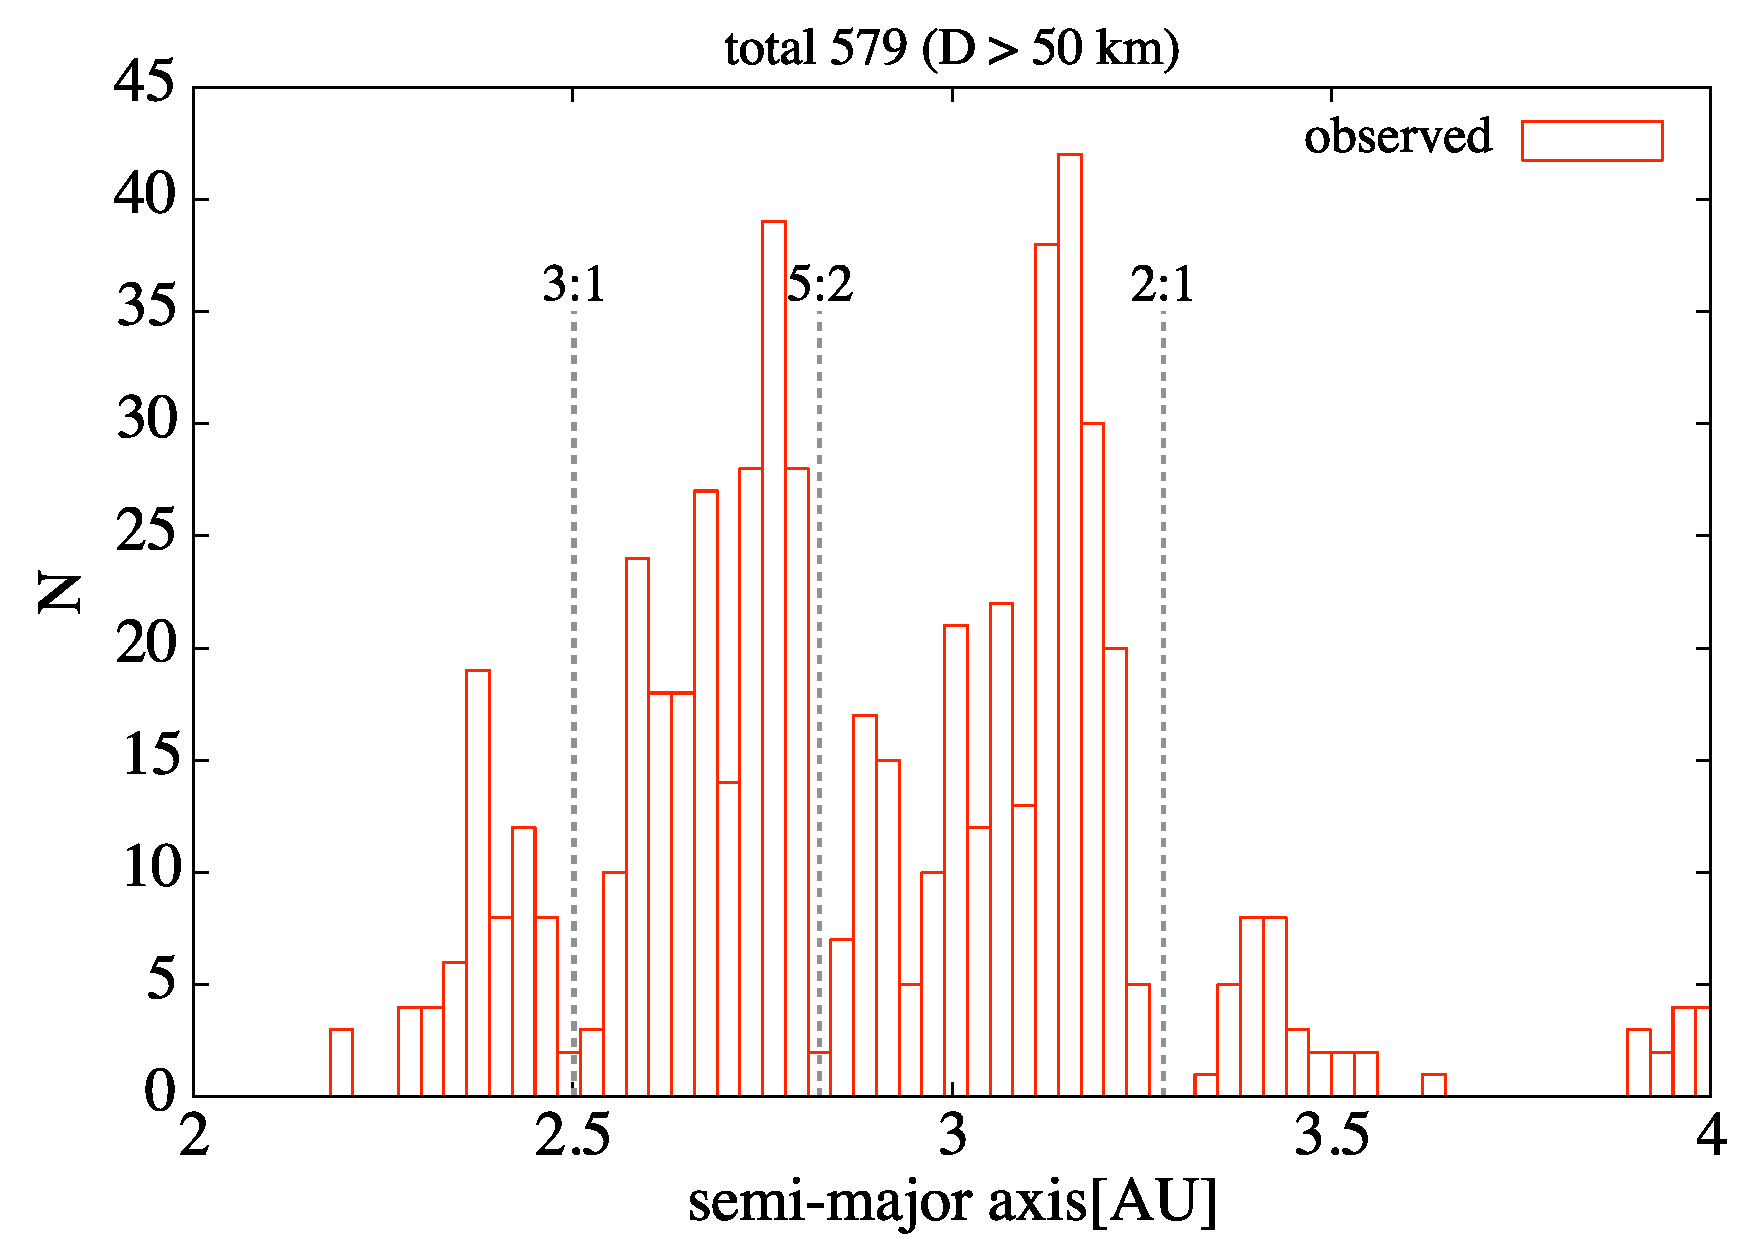
\includegraphics[width=8cm]{./image/mainbelt_histogram.pdf}
\end{minipage} &
%調整
\begin{minipage}[t]{0.1\hsize}
\end{minipage} &
%右
\begin{minipage}[t]{0.45\hsize}
\centering
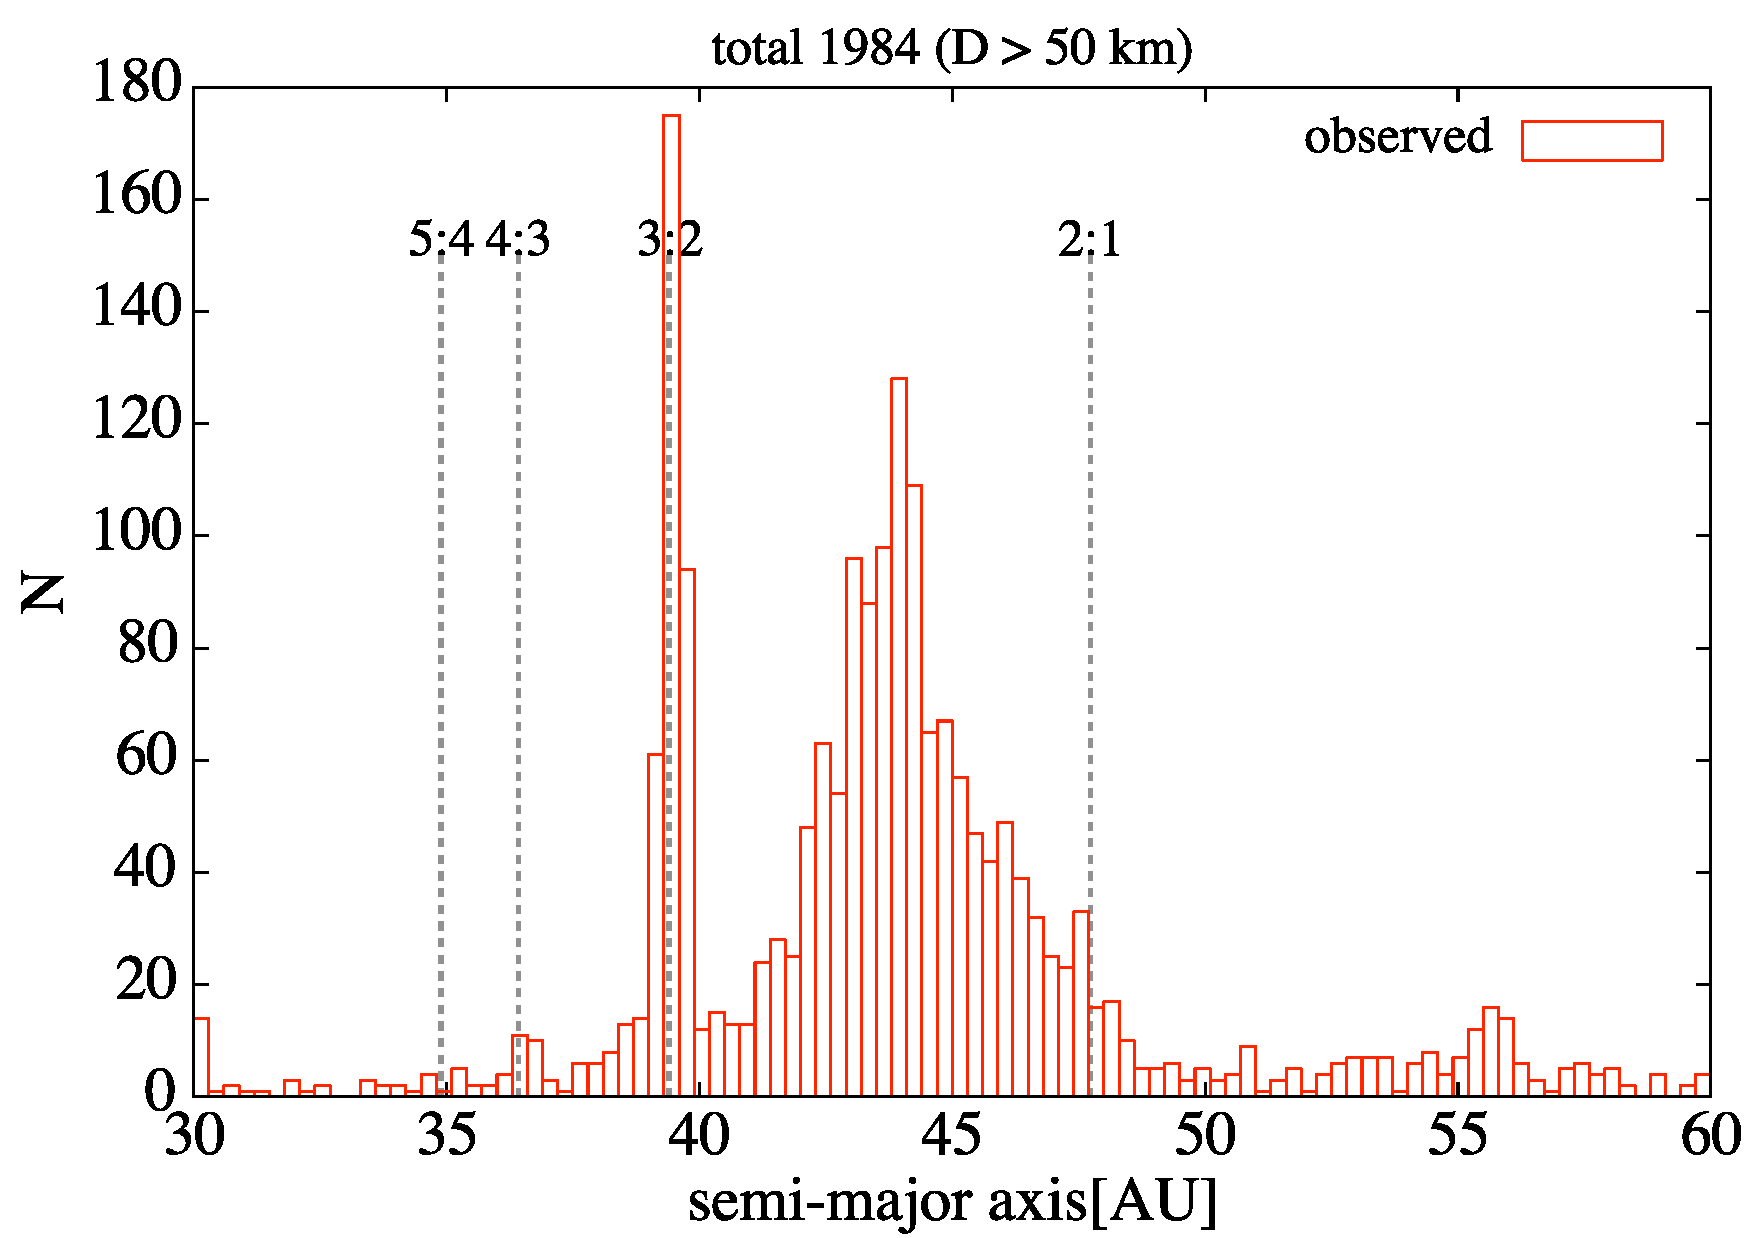
\includegraphics[width=8cm]{./image/kuiperbelt_histogram.pdf}
\end{minipage}\\
%
\end{tabular}
\caption{小惑星帯領域(左)とカイパーベルト領域(右)の小天体の軌道長半径に対する個数分布.\label{fig:obs_histogram}}
\end{figure}


一方カイパーベルトでは,3:2の尽数関係の位置で0.1から0.3までに集中しており,また3:2と2:1の尽数関係の間の領域では0から0.2までに集中している.さらに,大多数の小天体が海王星と軌道交差しない領域にいる中で,3:2の尽数関係の位置には軌道交差しているものが比較的多く存在する(図 \ref{fig:obs_ecc} 右参照).

\begin{figure}[H]
\begin{tabular}{ccc}
%左
\begin{minipage}[t]{0.45\hsize}
\centering
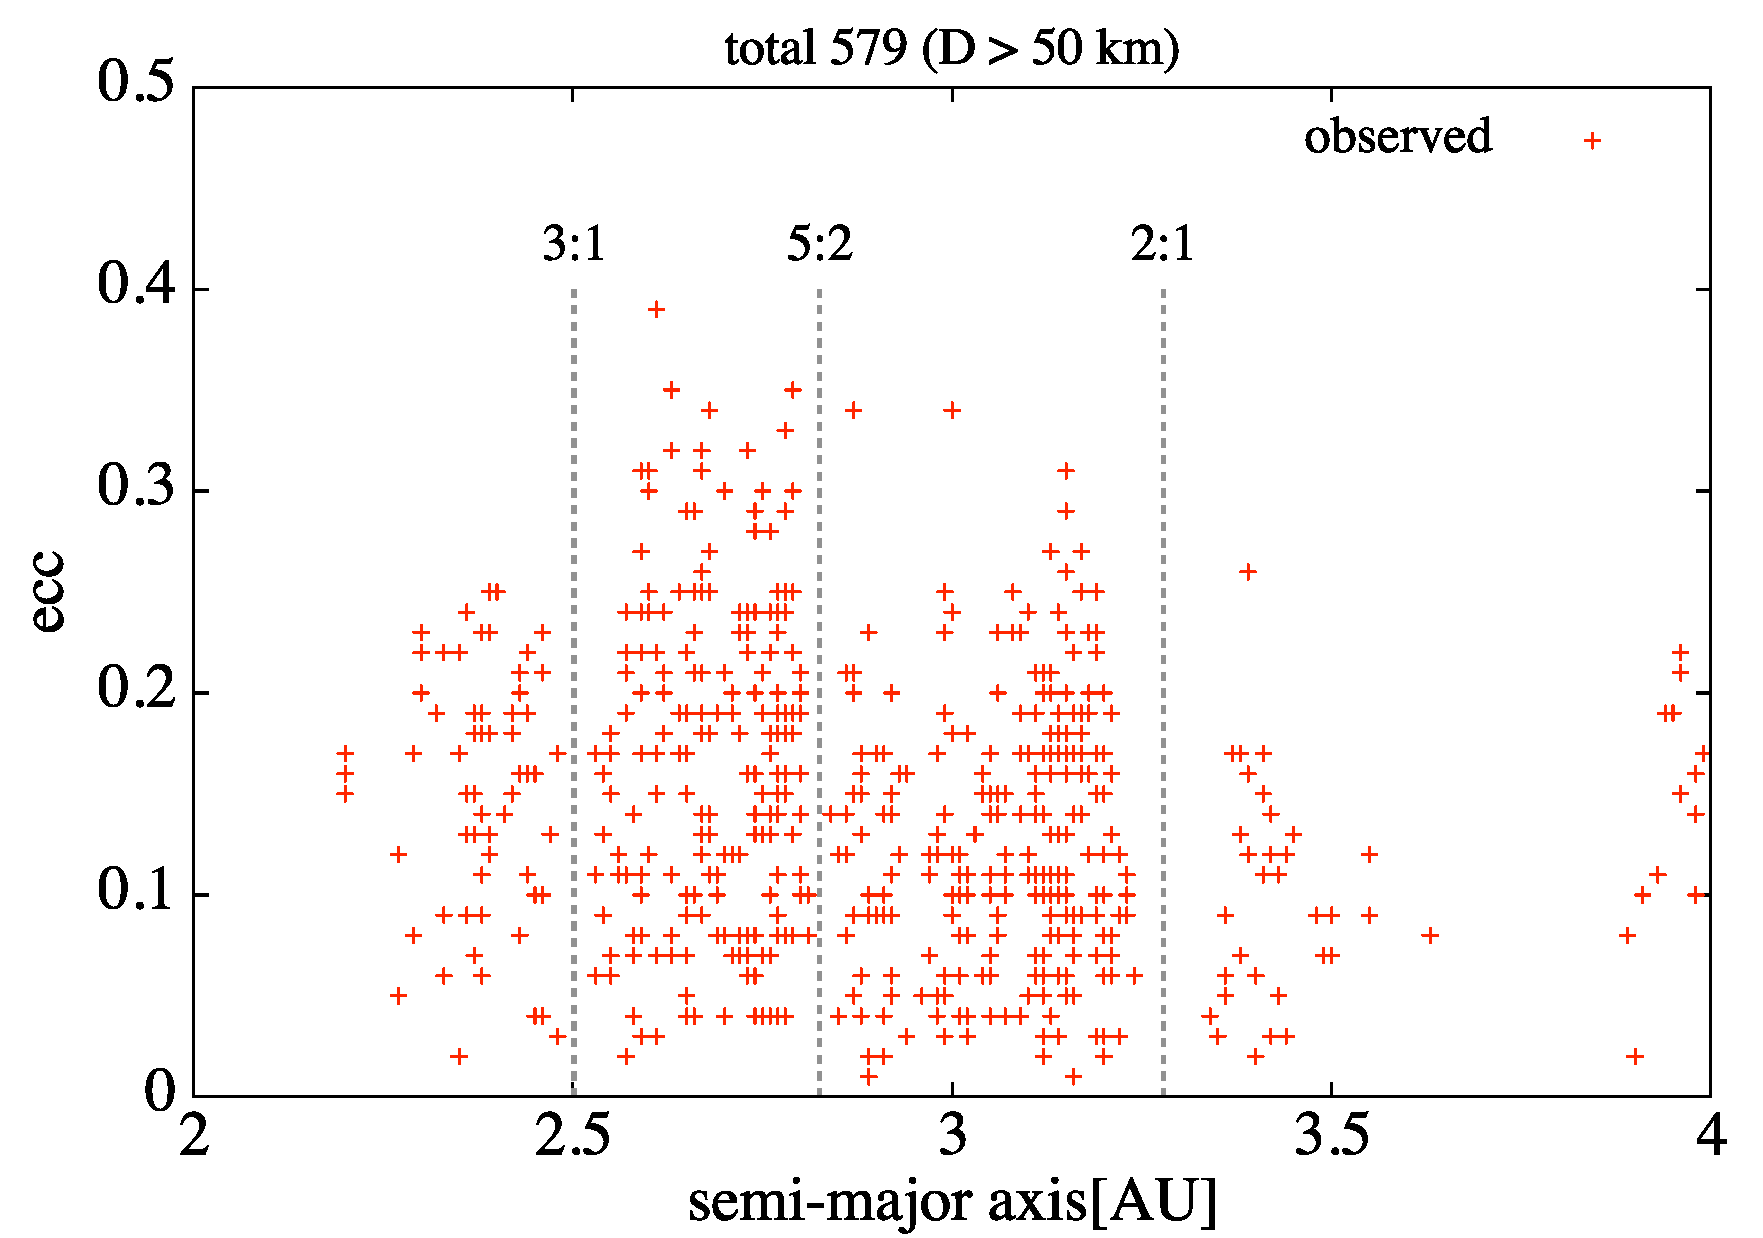
\includegraphics[width=8cm]{./image/mainbelt_ecc.pdf}
\end{minipage} &
%調整
\begin{minipage}[t]{0.1\hsize}
\end{minipage} &
%右
\begin{minipage}[t]{0.45\hsize}
\centering
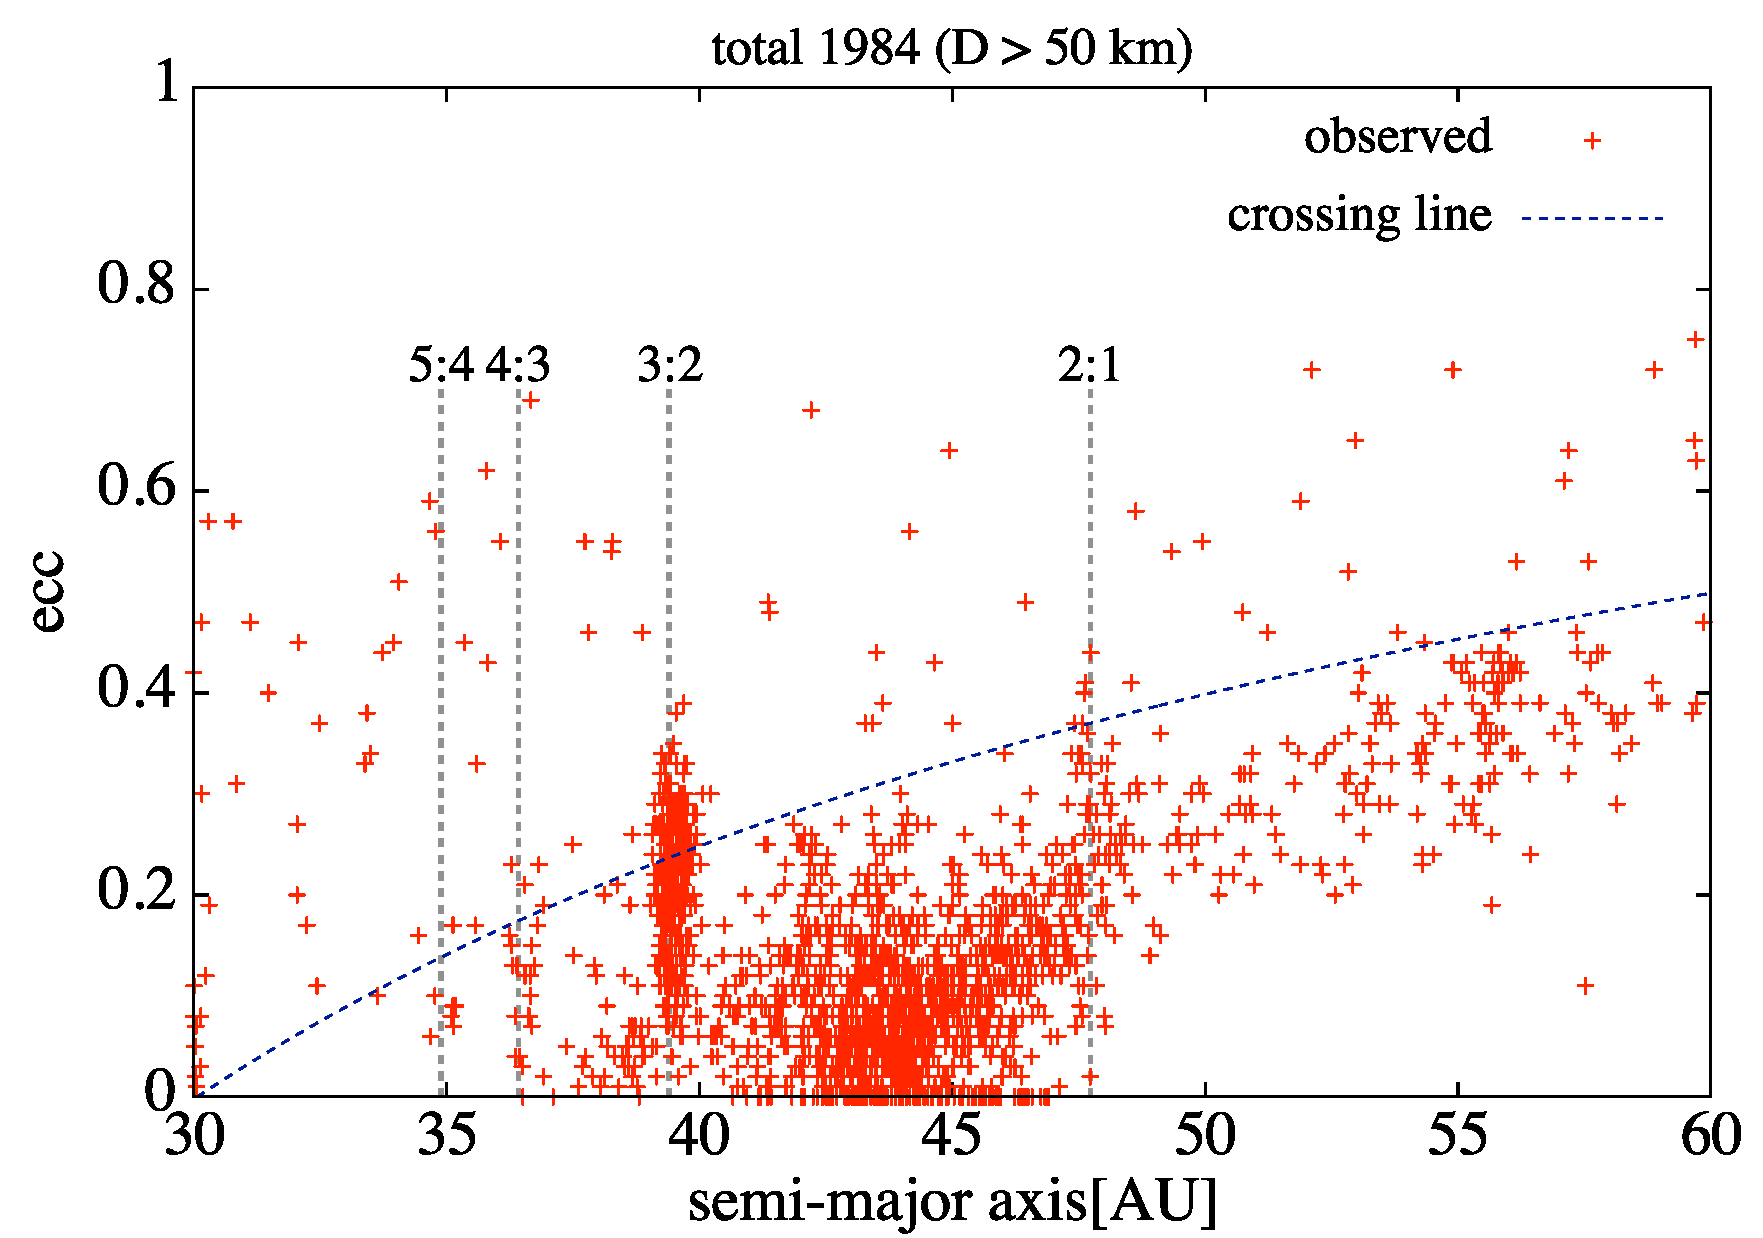
\includegraphics[width=8cm]{./image/kuiperbelt_ecc.pdf}
\end{minipage}\\
%
\end{tabular}
\caption{小惑星帯領域(左)とカイパーベルト領域(右)の小天体の離心率.また近日点距離が $30 {\rm AU}$ と一致するときの,軌道長半径と離心率の関係を曲線で表している.\label{fig:obs_ecc}}
\end{figure}


これらの運動方程式はスカラー関数 $U$ の勾配として書くこともできる.
\begin{eqnarray}
\ddot{x} - 2 n \dot{y} & = & \frac{\partial U}{\partial x}, \label{eq:xU}\\
\ddot{y} + 2 n \dot{x} & = & \frac{\partial U}{\partial y}, \label{eq:yU}\\
\ddot{z} & = & \frac{\partial U}{\partial z}. \label{eq:zU}
\end{eqnarray}
ここで $U = U (x, y, z)$ は次のように与えられる.
\begin{equation}
U = \frac{n^2}{2} (x^2 + y^2) + \frac{\mu_1}{r_1} + \frac{\mu_2}{r_2}. \label{eq:U}
\end{equation}
$x^2 + y^2$ の項は遠心力によるポテンシャル,$1/r_1, 1/r_2$ の項は重力によるポテンシャルであり,それぞれの偏微分をとると運動方程式に遠心力,重力の項が現れる.

(\ref{eq:xU}),(\ref{eq:yU}) 式の $- 2n \dot{y}$ と $+ 2n \dot{x}$ の項はコリオリ項であり,回転座標系での粒子の速度に依存する.コリオリ力は速度方向に対して右側にずれる力であり,ゆえに効かない.



\small{
\begin{thebibliography}{99}
\bibitem{A}
はてなブログで TeX 表記する方法による見た目を比較 - joker8phoenix's diary, 
\url{http://joker.hatenablog.com/entry/2013/06/06/074105}
\end{thebibliography}

}
\end{document}